\documentclass[12pt]{article}
\usepackage[left=0.25cm,top=1cm,right=0.25cm,bottom=1cm]{geometry}
\textwidth = 20cm
\hoffset = -1cm
\usepackage[utf8]{inputenc}
\usepackage[spanish,es-tabla]{babel}
\usepackage[autostyle,spanish=mexican]{csquotes}
\usepackage[tbtags]{amsmath}
\usepackage{nccmath}
\usepackage{amsthm}
\usepackage{amssymb}
\usepackage{graphicx}
\usepackage{standalone}
\usepackage[outdir=./]{epstopdf}
\usepackage{siunitx}
\usepackage{physics}
\usepackage{color}
\usepackage{float}
\usepackage{multicol}
%\usepackage{milista}
\usepackage{enumitem}
\usepackage{anyfontsize}
\usepackage{anysize}
\usepackage{enumitem}
\usepackage{capt-of}
\usepackage{bm}
\usepackage{relsize}
\usepackage{placeins}
\usepackage{empheq}
\usepackage{cancel}
\usepackage{wrapfig}
\spanishdecimal{.}
\renewcommand{\baselinestretch}{1.5} 
\renewcommand\labelenumii{\theenumi.{\arabic{enumii}}}
\newcommand{\ptilde}[1]{\ensuremath{{#1}^{\prime}}}
\newcommand{\stilde}[1]{\ensuremath{{#1}^{\prime \prime}}}
\newcommand{\ttilde}[1]{\ensuremath{{#1}^{\prime \prime \prime}}}
\newcommand{\ntilde}[2]{\ensuremath{{#1}^{(#2)}}}


\geometry{top=1.25cm, bottom=1.5cm, left=1.25cm, right=0.8cm}
%\usepackage{showframe}
\title{Examen Tarea Tema 4 \\ \large {Matemáticas Avanzadas de la Física}  \vspace{-3ex}}
\author{M. en C. Gustavo Contreras Mayén}
\date{ }
\begin{document}
\vspace{-4cm}
\maketitle
\fontsize{14}{14}\selectfont
\begin{enumerate}
\item Expande en términos de una serie con Polinomios de Legendre los siguientes polinomios:
\begin{enumerate}
\item $3 \, x^{2} + x - 1$
\item $x - x^{3}$
\end{enumerate}
\item Calcula el potencial electrostático del arreglo de cargas que se muestra en la figura (\ref{fig:figura_octupolo}). Éste es un ejemplo de dos dipolos iguales pero dirigidos de manera opuesta. Las contribuciones por los dipolos se cancelan. Los términos del octupolo no se cancelan.

\begin{figure}[H]
    \centering
    \includegraphics[scale=1.3]{Imagenes/octupolo_1.eps}
    \caption{Octupolo lineal eléctrico.}
    \label{fig:figura_octupolo}
\end{figure}

\item La amplitud de una onda dispersada está dada por
\begin{align*}
f(\theta) = \dfrac{1}{k} \, \sum_{\ell = 0}^{\infty} (2 \, \ell + 1) \, \exp(i \, \delta_{\ell}) \, \sin \delta_{\ell} \, P_{\ell} (\cos \theta)
\end{align*}
Donde $\theta$ es el ángulo de dispersión, $\ell$ es el valor propio del momento angular, $\hbar \, k$ es el momento incidente, y $\delta_{\ell}$ es el desplazamiento de fase producido por el potencial central que está haciendo la dispersión. La sección transversal total es 
\begin{align*}
\sigma_{\text{tot}} = \int \abs{f(\theta)}^{2} \dd{\Omega}
\end{align*}
Demuestra que
\begin{align*}
\sigma_{\text{tot}} = \dfrac{4 \, \pi}{k^{2}} \sum_{\ell=0}^{\infty} (2 \, \ell + 1) \, \sin^{2} \delta_{\ell}
\end{align*}
\item Una esfera conductora de calor de radio $a$ está compuesta por dos hemisferios con un espacio infinitesimal aislante entre ellos, como se muestra en la figura (\ref{fig:figura2}). Las mitades superior e inferior de la esfera están en contacto con baños térmicos de temperaturas $+ T_{1}$ y $-T_{1}$, respectivamente. La esfera de radio $a$ está dentro de otra esfera conductora de calor de radio $b$ con una temperatura $T_{2}$.

Calcula la temperatura en los puntos:
\begin{enumerate}
\item Dentro de la esfera interior,
\item En la región entre las dos esferas y
\item Por fuera de la esfera exterior.
\end{enumerate} 
\begin{figure}[!ht]
    \centering
   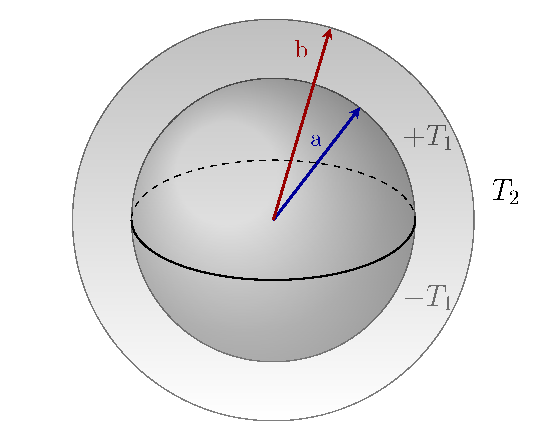
\includegraphics[scale=0.8]{Imagenes/esfera1.eps}
    \caption{Los hemisferios de la esfera interior se encuentran a diferentes temperatura.}
    \label{fig:figura2}
\end{figure}
\item En la figura (\ref{fig:esfera_aterrizada}) se muestra una esfera de radio $a$ con un pequeño espacio aislante en su ecuador, la semiesfera inferior se encuentra aterrrizada, mientras que la semiesfera superior se mantiene a un potencial constante $V_{0}$. Calcula el potencial electrostático en puntos dentro de la esfera.
\begin{figure}[!ht]
    \centering
   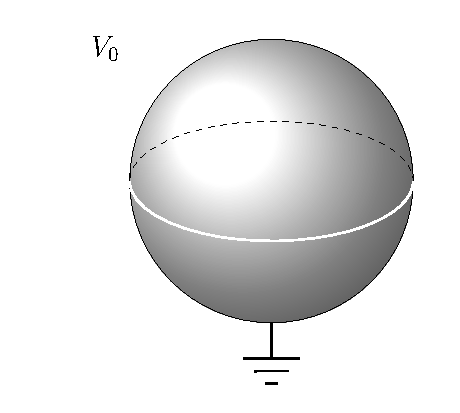
\includegraphics[scale=0.8]{Imagenes/esfera_5.eps}
    \caption{El semihemisferio inferior se encuentra aterrizado.}
    \label{fig:esfera_aterrizada}
\end{figure}
\end{enumerate}
\end{document}